\documentclass[11pt]{article}

\usepackage[portuguese]{babel}
\usepackage[T1]{fontenc}
\usepackage[utf8]{inputenc}
\usepackage{amsmath}
\usepackage{graphicx}
\usepackage{subfig}
\usepackage[colorinlistoftodos]{todonotes}
\usepackage{listings}
\usepackage{color} 
\usepackage{float}
\usepackage[font={footnotesize}]{caption}
\usepackage{xcolor,colortbl}
\usepackage{array}
\usepackage{fixltx2e}


%lslist pra por codigo no latex?

\linespread{1.3}
\usepackage{indentfirst}
\usepackage[top=2cm, bottom=2cm, right=2.5cm, left=2.5cm]{geometry}

\begin{document}
	
\begin{titlepage}
	\begin{center}
		
		\hfill \break
		\hfill \break
		
		
\includegraphics[width=0.3\textwidth]{./logo}~\\[1cm]
		
		\textsc{\Large Mestrado Integrado em Engenharia Electrotécnica e de Computadores}\\[1.5cm]
		\textsc{\huge Sistemas Electrónicos de Processamento de Sinal}\\[0.25cm]
		
		{\huge \bfseries BPSK Modem \\[1.2cm]}
		
		Grupo n.º 2/3 \vspace{0.3cm}
		
		\begin{tabular}{l r}
			André Filipe Barroso Cerqueira \hspace{1mm} & n.º 65144 \\
			Guilherme Branco Teixeira \hspace{1mm} & n.º 70214  \\
			João André Catarino Pereira & n.º 73527
		\end{tabular}
		
		\hfill
		\hfill
		
		segunda-feira 15h30 - 18h30, LE1
		
		\vfill
		
		{\large Lisboa, 11 de Abril de 2015} 
		
	\end{center}
\end{titlepage}

\section{Índice}

\section{Introdução}

-objectivos do lab  

-o que foi feito

-o q o relatorio vai falar



\section{Projecto}

\subsection{Projectos de Demonstração}
-Resumo das funçoes e os seus objectivos com especial importancia ao loop

-Relaciona-las com as suas utilizaçoes no projecto em si

\subsubsection{sine8}
O objectivo deste projeto é representar a função sinusoidal, multiplicada por um determinado ganho, através de um conjunto de amostras que equivalem a um período da mesma, repetindo nos períodos seguintes esse mesmo conjunto. Este procedimento é realizado através da rotina de interrupção presente no programa. 

Ao analisar o código deste projeto à primeira vista podemos concluir logo que este usa uma frequência de amostragem de 8 kHz , tem um ganho $G=10$ predefinido e usa 8 amostras para representar a sinusoide. Depois de observar a sinusoide no osciloscópio variou-se o ganho a fim de perceber a sua influência e também o seu limite.
 
Para compreender o limite desta sinusoide é necessário ter em conta que se usa o formato de vírgula fixa Q15 para as amostras da sinusoide. Este formato tem como limite o valor $(2^{15}-1) = 32767$. Considerando o valor máximo da sinusoide, se multiplicarmos a mesma por um ganho G=33 obtemos um valor superior ao permitido pelo formato Q15, fazendo com que nesses pontos o valor da sinusoide "caia".     

\subsubsection{loop}
Este projeto tem como objectivo fornecer-nos um template para os próximos projetos, em termos de comunicação com a placa e rotina de interrupção. Pode-se observar nas últimas linhas de código como se liga os sinais de entrada e saída aos canais da placa.

Resultados do loop??

\subsection{BPSK}

 Demonstração dos Resultados usando como etapas as varias perguntas do enunciado, complementar com as fotos e possiveis tabelas ou partes de codigo

\subsubsection{P1. Oscilador controlado numericamente}

%fazer espectros e comparar!!!

\subsubsection{P2. Transmissor BPSK}

%Introdução Teórica
O objectivo deste projeto é criar um transmissor BPSK com recurso a três elementos principais, uma fonte de bits, um codificador diferencial e mapeador, e um modulador.
Neste projeto foi utilizada uma frequência de amostragem $fs=16kHz$ e uma frequência portadora $f_0=4kHz$.
%COMPLEMENTAR com alguma teoria

%Pergunta 1
Para ter uma fonte de bits no transmissor usa-se um "bit-rate clock", cuja função vai ser criar uma sequência de bits $ b_n $ que a cada 16 ciclos gera um novo bit alternado, usando um contador com $fs/16$ para determinar quando gerar um novo bit. Para alternar o bit basta negar o bit anteriormente obtido, o que foi concretizado através de uma simples XOR:
\begin{equation}
b_n=b_{n-1} \oplus 1
\end{equation}
Após obter a fonte de bits passa-se ao segundo elemento do transmissor, o codificador diferencial e mapeador. Começando pelo codificador diferencial, este utiliza bn para aplicar a seguinte operação lógica:
\begin{equation}
c_n=c_{n-1} \oplus b_n
\end{equation}
Assim, com $c_0$ inicializado a zero codifica-se a sequência de bits $ b_n $. Ao gerar $ b_n $ e $ c_n $ obtém-se dois sinais que variam entre "0" e "1" só que $ c_n $ tem o dobro do período (figura X).
\begin{figure}[h]
	\centering
	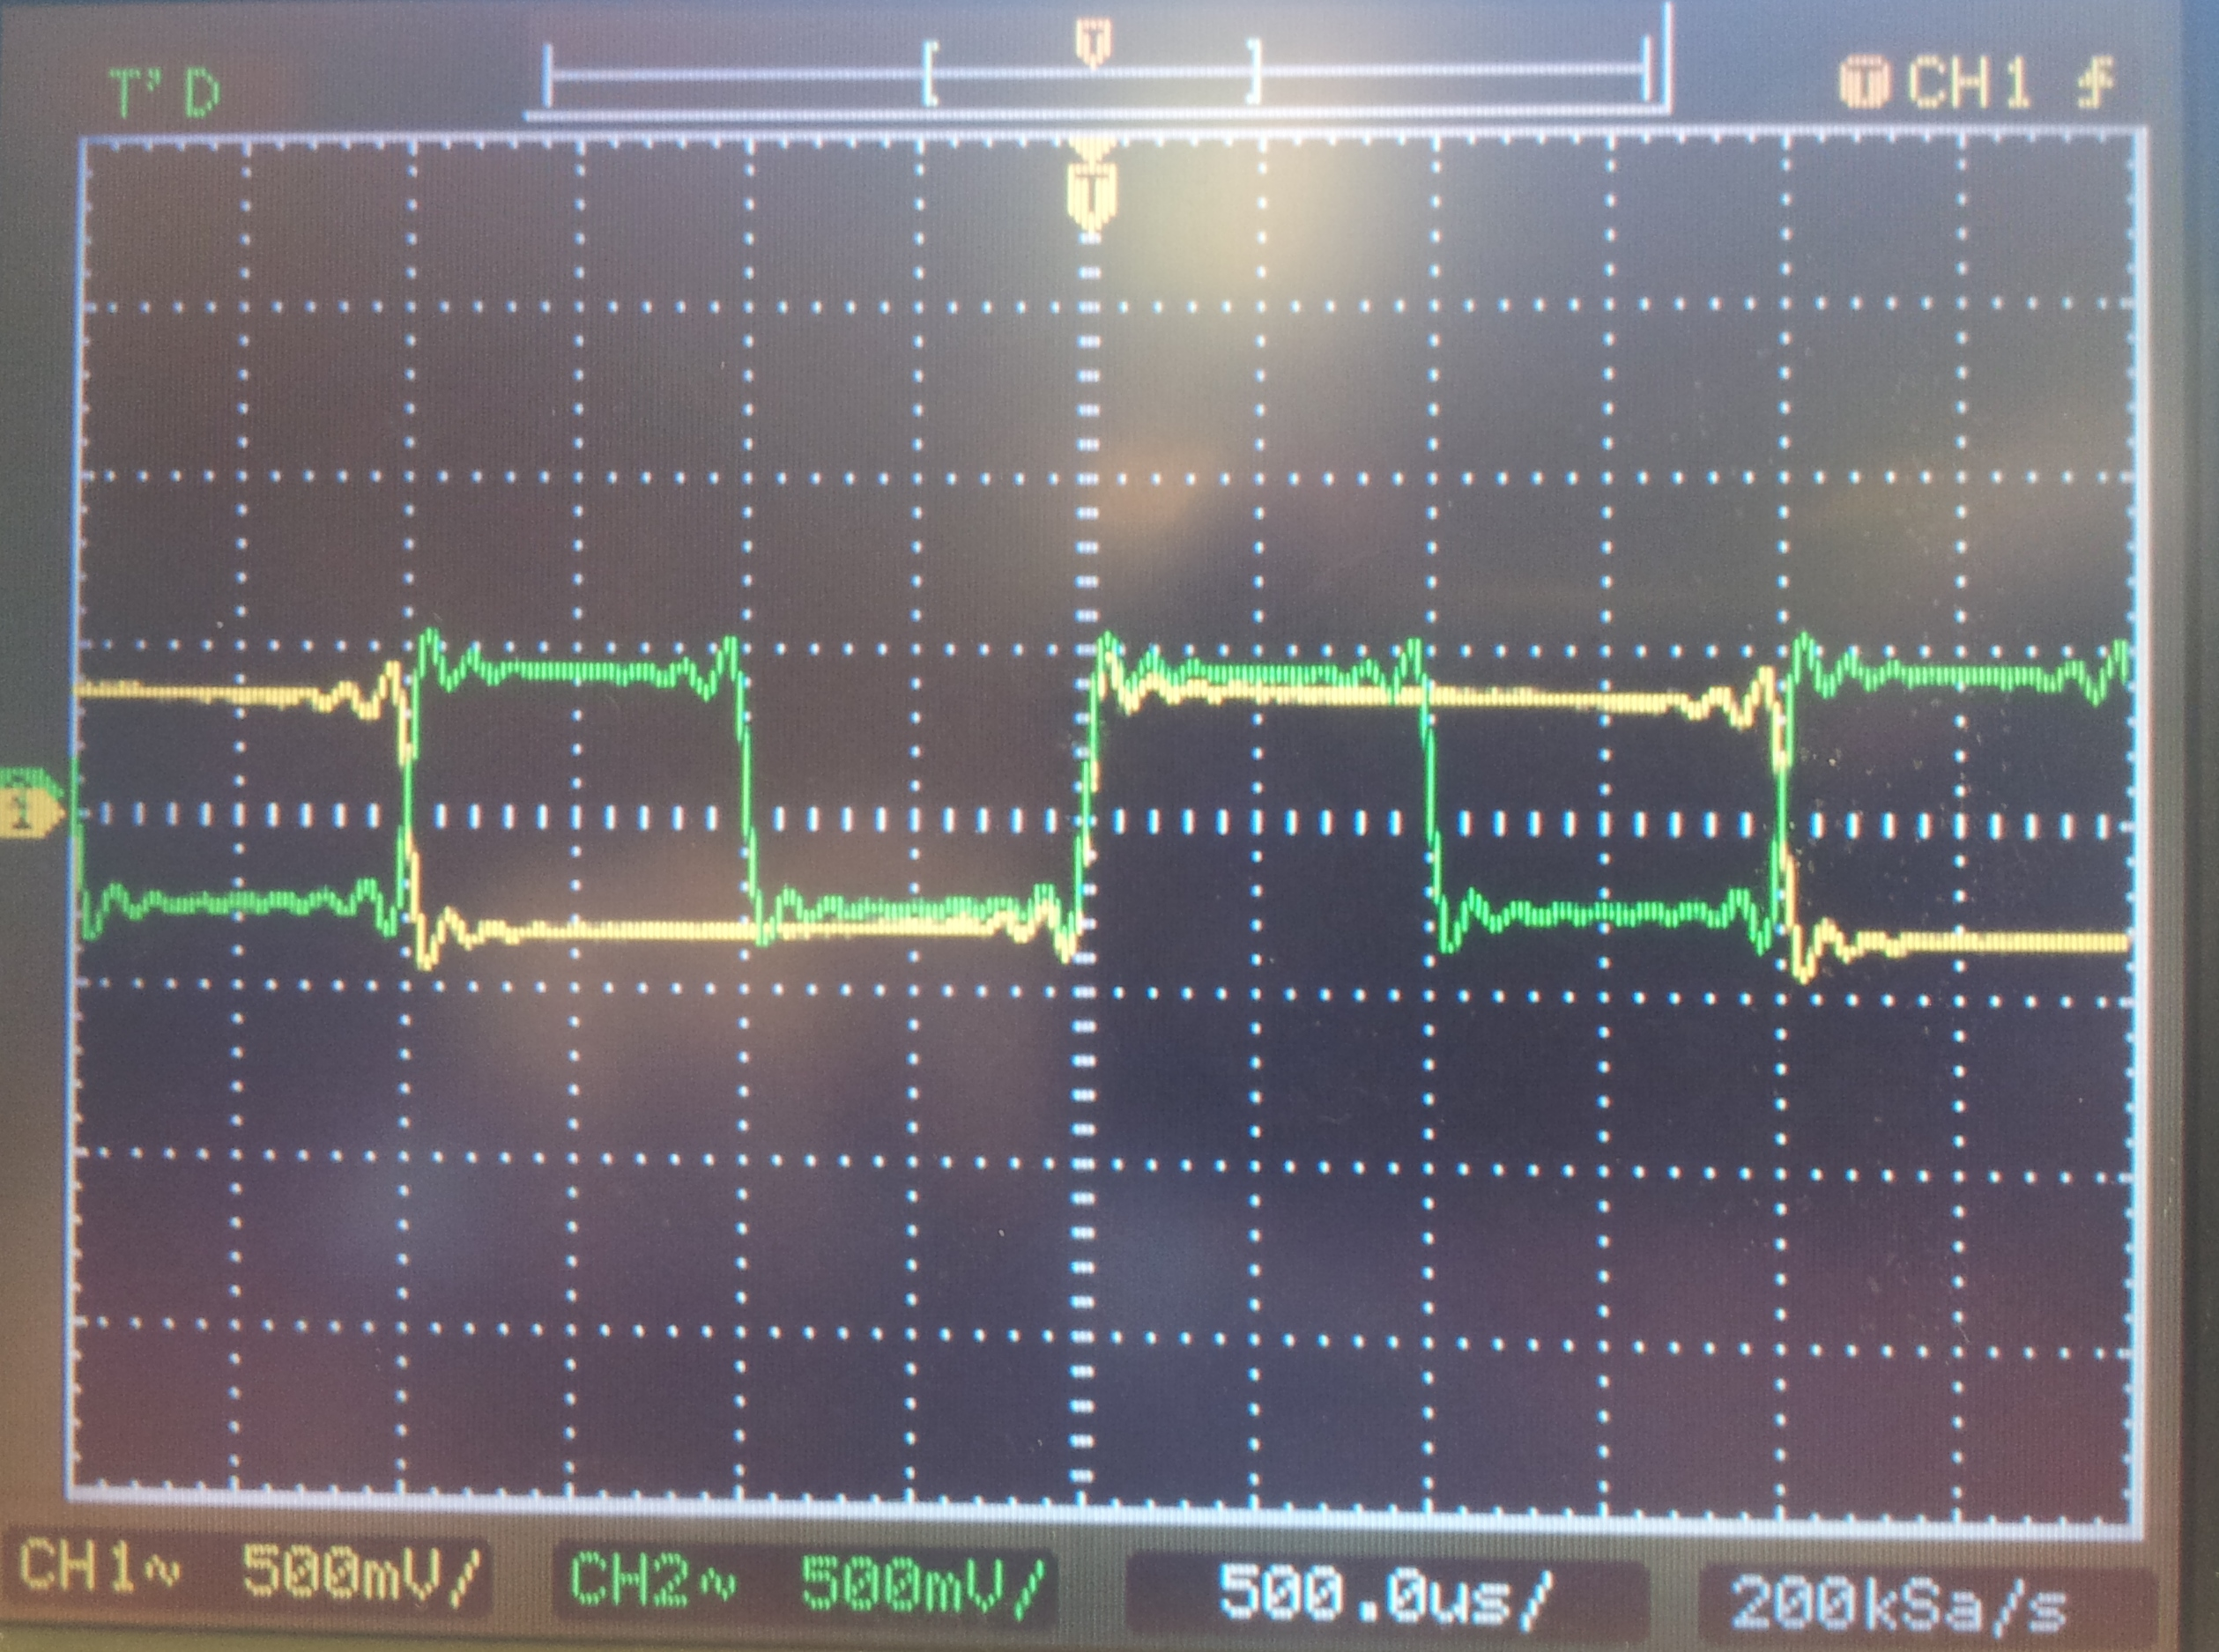
\includegraphics[width=0.5\textwidth]{./bn_cn}~\\
	\caption{$ b_n $(verde) e $ c_n $(amarelo)}
\end{figure}

\vspace{-0.4cm}
Depois de obter $ c_n $ passa-se ao mapeamento do mesmo,
%explicar f=500Hz
%complementar com o que?

%Pergunta 2

%Pergunta 3

%Explicar FFT!!!

\section{Conclusão}
-Principais resultados e conclusoes sobre eles, erros a corrigir (se houverem), o que melhorar

\section{Anexos}
-Codigo?

-possivelmente poe-se aqui algumas das imagens	
\end{document}